% Intended LaTeX compiler: pdflatex
\documentclass[10pt,a4paper,UTF8]{article}
\usepackage{zclorg}
\usepackage{tikztheorem}
\author{Eastern(ZCL)}
\date{}
\title{802.11a峰值速率计算}
\hypersetup{
 pdfauthor={Eastern(ZCL)},
 pdftitle={802.11a峰值速率计算},
 pdfkeywords={},
 pdfsubject={},
 pdfcreator={Emacs 25.0.50.1 (Org mode 9.1.2)},
 pdflang={English}}
\begin{document}

\maketitle
\tableofcontents
\titlepic{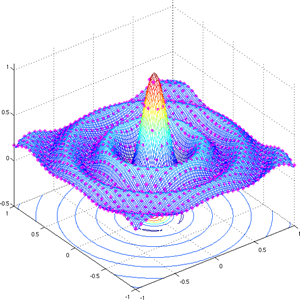
\includegraphics[scale=0.25]{../../img/sinc.PNG}}
IEEE802.11a可以支持8种速率模式。

IEEE802.11a的OFDM符号保护间隔长度是800ns,实际系统中传输保护间隔是需要能量的。为了把保护间隔所占的功率减小到1dB,OFDM符号的长度定位\$4\(\mu\) s\$。这样出去保护间隔,有效数据部分长度为\(3.2\mu s\),进而可以得到子载波间隔为\$\frac{1}{3.2 \mu s}= 312.5kHz\$。IEEE802.11a采用48个并行子载波进行数据传输,这样当调制方式为BPSK或者16QAM时,可以提供的未编码数据速率分别为\$48\texttimes{} 1\texttimes{} \frac{1}{4 \mu s}= 12Mbps\$和\$48\texttimes{} 4\texttimes{} \frac{1}{4 \mu s}= 48Mbps\$。同时为了兼顾有效性和可靠性,协议规定根据信道状况不同可以采用不同编码效率的卷积编码在各个子信道之间进行卷积编码。基本的编码效率是1/2,可以通过打孔的方式实现2/3,3/4的编码效率。这样四种调制方式采用BPSK,QPSK,16QAM,64QAM。每一种调制方式配合两种码率的编码方式,就产生了协议支持的八种速率模式。最终结果如下图所示。

\begin{center}
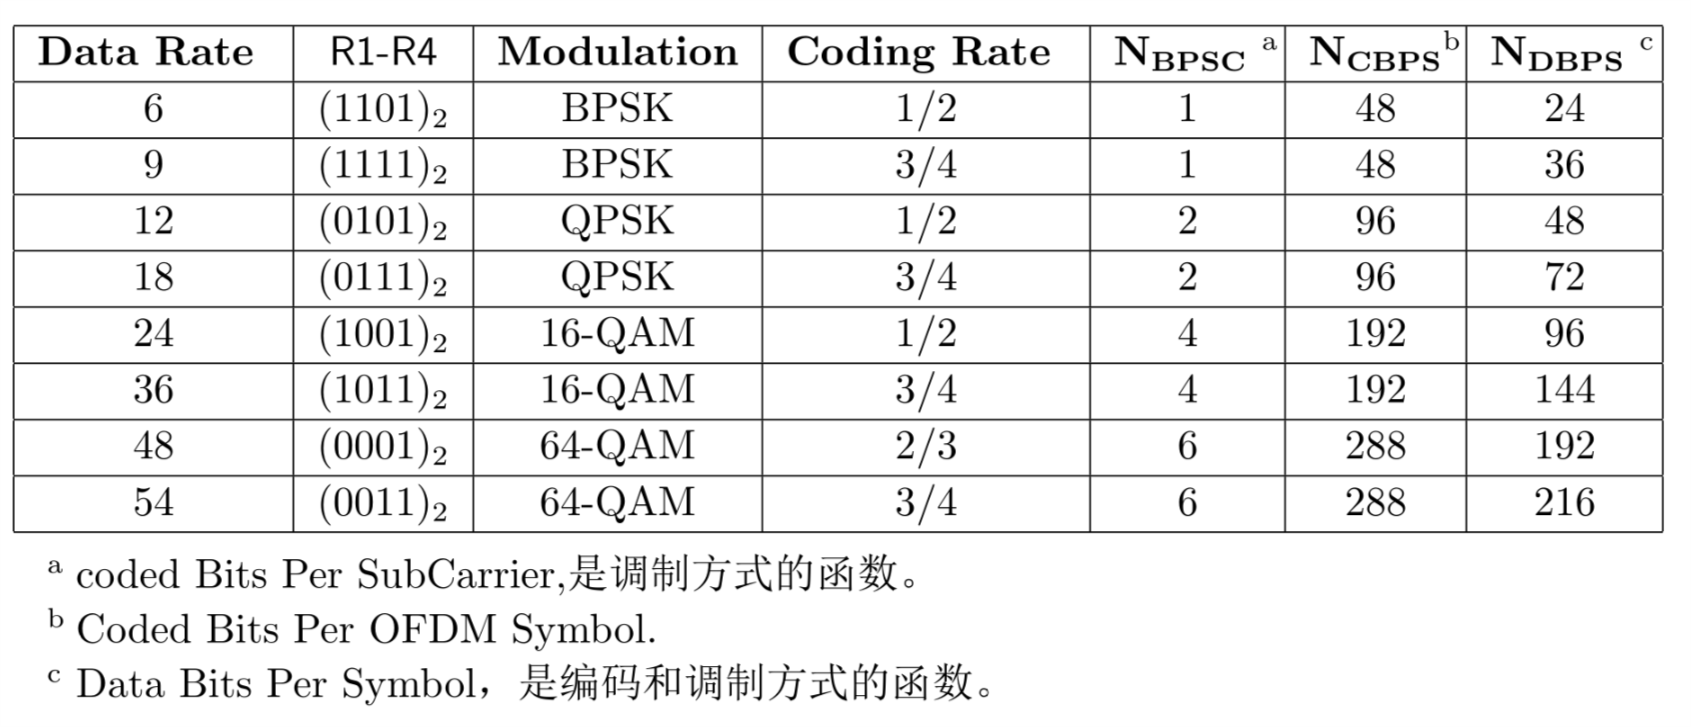
\includegraphics[width=.9\linewidth]{../../img/communication_protocol/20171018wifiPeakRate.png}
\end{center}


表格中的第二列是这八种速率模式在协议的PLCP帧头的SIGNAL区域中二进制表示。\\

在IEEE802.11a中使用了53个子载波传送数据(48个数据子载波,4个导频子载波,一个零频子载波)。但是为了方便IFFT的计算采用了64点IFFT计算,设置总子载波个数是64。在53个子载波的标号低端和标号高端分别插入6个和5个零符号。这样做的好处有:1)保证了子载波个数是2的幂次,做IFFT计算很方便。2)插入的11个零符号子载波可以作为保护间隔,以防其他信道的信号造成干扰。52个非零子载波的映射如下图所示,这中映射方式在matlab中可以使用函数ifftshift()实现。


\begin{center}
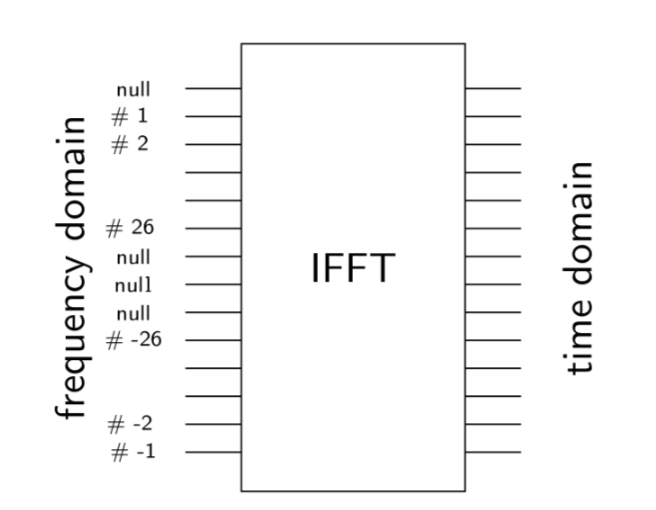
\includegraphics[width=.9\linewidth]{../../img/communication_protocol/20171018fft54.png}
\end{center}

频域数据经过IFFT计算后转化到时域。在IEEE802.11a中,PPDU传输的时间--频域分布图,如下图所示。

\begin{center}
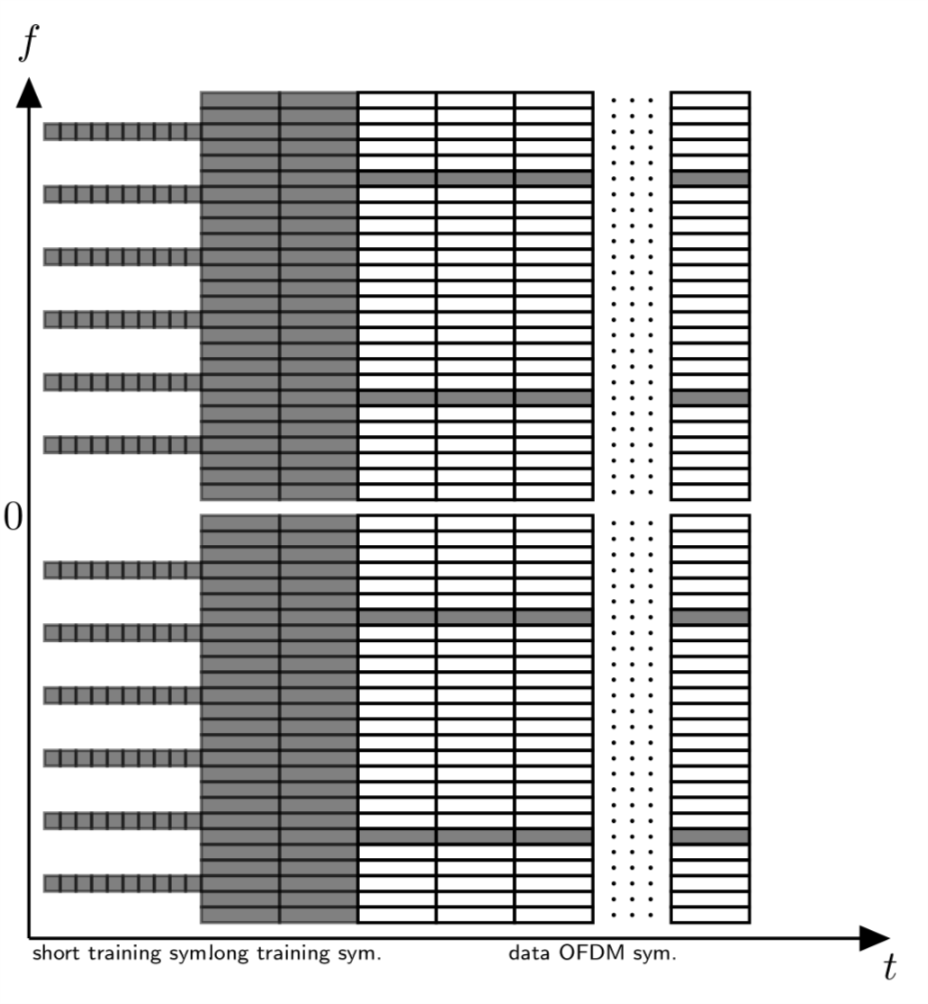
\includegraphics[width=.9\linewidth]{../../img/communication_protocol/20171018ppdu.png}
\end{center}

由于在实际运算中,64个数据送入IFFT是按照上图进行映射的,但是协议在计算短训练符号和长训练符号过程中其频域数据都是以\$l\_\{-26,26\}\$或者\$L\_\{-26,26\}\$的形式给出的,也就是说计算IFFT时需要把标号为负的子载波放到IFFT输入数据标号较大的位置,这样在进行matlab仿真过程中就需要把短训练序列和长训练序列的频域形式进行翻转,这一过程可以使用ifftshift()或者fftshift()方便的实现。\\

在生成数据OFDM符号的过程中,基带发射机接收经过星座映射并加入导频的复数,然后把这些52个数加上一个零频和11个空符号(48个复数头部添加6个,尾部添加5个,这些空符号做保护子载波使用)送入IFFT。这48个复数的编号从0到47,要把其按照式(\ref{eq:2011041901})映射到以零频为中心的正负子载波两边。
\begin{equation}
M(k)= \left\{ \begin{array}{ll}
  k-26 & \textrm{$\quad 0\leq k\leq 4$}\\
  k-25 & \textrm{$\quad 5\leq k\leq 17$}\\
  k-24 & \textrm{$\quad 18\leq k\leq 23$}\\
  k-23 & \textrm{$\quad 24\leq k\leq 29$}\\
  k-22 & \textrm{$\quad 30\leq k\leq 42$}\\
  k-21 & \textrm{$\quad 43\leq k\leq 47$}
  \end{array} \right.
 \label{eq:2011041901}
\end{equation}
实际上,星座图映射结束加上四个导频后得到的52个复数默认的就是从-26到26,即他们的位置就是正确的子载波位置,只不过编号不是从0到52而是从-26到26。子载波编号和IFFT输入编号的映射问题在写matlab程序中需要注意协议的唯一一点要求是要调用ifftshift()函数。经过ifftshift()函数,自载波编号\$-26,-25,\ldots,-2,-1,1,2,\ldots,25,26\$被映射为\$0,1,2,\ldots,26,-26,-25,-24,\ldots,-2,-1\$。当然残余映射的还有分别加在52个复数头部、中间和尾部的6个空符号、直流零频和5个空符号,这样每一个OFDM符号子64个子载波的频域波形框架如下图 。图中标有d的子载波是数据子载波,标有v的子载波是虚子载波,标有p的子载波是导频子载波。最终输入IFFT进行运算的数据编号如下图所示。

\begin{center}
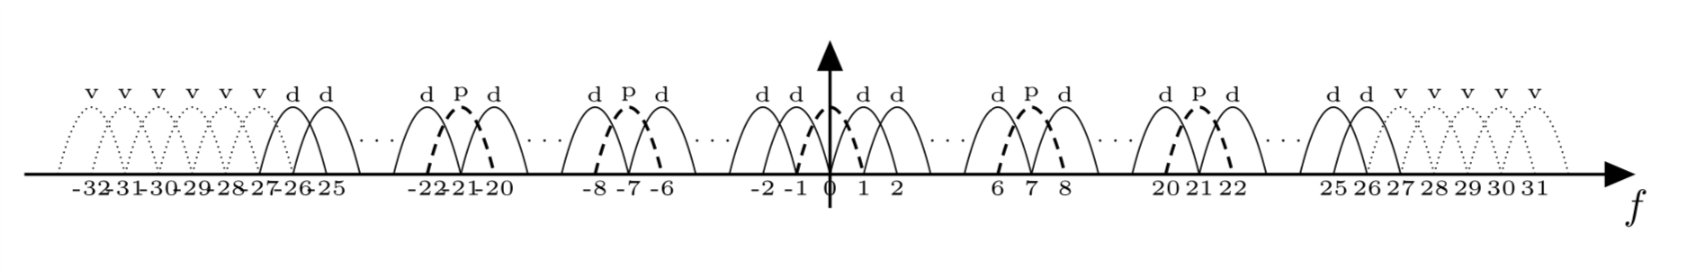
\includegraphics[width=.9\linewidth]{../../img/communication_protocol/2017101864fft.png}
\end{center}
\end{document}
